\chapter{DESARROLLO DEL PROYECTO}

Se pone a consideraci\'{o}n los siguientes objetivos espec\'{i}ficos:

\begin{itemize}

\item Proveer personalizaci\'{o}n de servicio agregador de noticias por programa
de aprendizaje (sub-categor\'{i}a)
\item Implementar mecanismos de transcripci\'{o}n de contenidos.
\item Proveer representaci\'{o}n de microformatos para transcripci\'{o}n de 
contenido.
\item Facilitar pruebas de servicio agregador de noticias, reproducci\'{o}n Audio,
reproducci\'{o}n Video.

\end{itemize}

\section{Servicio Agregador de Noticias}

Las siguientes Historias de Usuario se definen en el proceso de Ingenier\'{i}a de
Requerimientos de duraci\'{o}n del proyecto adscripci\'{o}n.  

\subsection{Tarjetas de Historias de Usuario}

Las Historias de Usuario se elaboran en base a deseos de Carrera LAEL y
gestionado por un Coordinador designado al proyecto adscripci\'{o}n, el mismo
que sugirio cambios de funcionalidades en el transcurso del tiempo.

% add history card 03
\begin{minipage}[b]{\hsize}\centering

\begin{tabular}{|l|l|l|}
\hline
                                                                                                                                             & \textbf{Tarjeta Historia de Usuario}                                                                                      &                                                                                                                       \\ \hline
ID Historia: 03                                                                                                                              & \begin{tabular}[c]{@{}l@{}}Nombre: Suscripción a un\\ Podcast de un Aprendiz \\ Autorregulado.\end{tabular}               & Fecha: 22/04/2014                                                                                                     \\ \hline
\multicolumn{3}{|l|}{Rol: Aprendiz Autorregulado.}                                                                                                                                                                                                                                                                                                                                               \\ \hline
\begin{tabular}[c]{@{}l@{}}Modificación de Historia Numero:\\ 05\end{tabular}                                                                & Iteración Asignada: 7,8,9, 11                                                                                             & Prioridad en Negocio: Medio                                                                                           \\ \hline
Tiempo Estimado Inicial: 20                                                                                                                  & Riesgo en Desarrollo: Bajo                                                                                                & Tipo de Historia: Funcional                                                                                           \\ \hline
\multicolumn{3}{|l|}{\begin{tabular}[c]{@{}l@{}}Descripción:\\ \\ Yo como usuario Aprendiz,Autorregulado deseo suscribirme a un Podcast de un \\ determinado idioma, tal que solo pinchar en el botón de suscripción (para,esto ya \\ no necesito ingresar mi correo electrónico).\end{tabular}}                                                                                                    \\ \hline
\multicolumn{3}{|l|}{\begin{tabular}[c]{@{}l@{}}Pre Condición:\\ \\ Usuario Autentificado.	\\ Contenido publicado.		Servidor\\ SMTP configurado.\end{tabular}}                                                                                                                                                                                                                                     \\ \hline
\multicolumn{3}{|l|}{\begin{tabular}[c]{@{}l@{}}Post Condición:\\ \\ Recibir mensajes en mi bandeja de,entrada de mi cuenta de correo.\end{tabular}}                                                                                                                                                                                                                                                \\ \hline
\multicolumn{3}{|l|}{\begin{tabular}[c]{@{}l@{}}Observaciones:\\ \\ La suscripción del usuario Aprendiz\\ Autorregulado le permite acceder solo a un producto, sin permitirle\\ dejar comentarios o interactuar de otra manera en la plataforma.\end{tabular}}                                                                                                                                      \\ \hline
\begin{tabular}[c]{@{}l@{}}.............................................\\ Msc. Lic. Vladimir Costas Juaregui\\ PROJECT MANAGER\end{tabular} & \begin{tabular}[c]{@{}l@{}}......................................\\ Lic. Manuel Camacho Arce\\ PRODUCT OWNER\end{tabular} & \begin{tabular}[c]{@{}l@{}}.....................................\\ Juan Omar Huanca Balboa\\ SCRUMMASTER\end{tabular} \\ \hline

\end{tabular}
\captionof{table}{Tarjeta Historia de Usuario 03}
\source{fuente: (Elaboraci\'{o}n Propia)}

\end{minipage}

% add user history card 57
\begin{minipage}[b]{\hsize}\centering

\begin{tabular}{|l|l|l|}
\hline
                                                                                                                                                     & \textbf{Tarjeta Historia de Usuario}                                                                                          &                                                                                                                           \\ \hline
ID Historia: 57                                                                                                                                      & \begin{tabular}[c]{@{}l@{}}Nombre: Personalización\\  Subscripcion Sub Categorias\end{tabular}                                & Fecha: 03/05/2015                                                                                                         \\ \hline
\multicolumn{3}{|l|}{Rol: Aprendiz Autorregulado/ Tutor/ Coordinador/ Administrador}                                                                                                                                                                                                                                                                                                                             \\ \hline
\begin{tabular}[c]{@{}l@{}}Modificación de Historia\\ Numero:\end{tabular}                                                                           & Iteración Asignada: 9, 10                                                                                                        & Prioridad en Negocio: Medio                                                                                               \\ \hline
Tiempo Estimado Inicial: 20                                                                                                                          & Riesgo en Desarrollo:                                                                                                         & Tipo de Historia: Funcional                                                                                               \\ \hline
\multicolumn{3}{|l|}{\begin{tabular}[c]{@{}l@{}}Descripción:\\ \\ Yo como usuario Aprendiz Autorregulado, Tutor, Coordinador, Administrador  deseo poder \\ personalizar mi subscripcion tal que me beneficie en poder escoger \\ mis intereses de subcategorias.\end{tabular}}                                                                                                                                     \\ \hline
\multicolumn{3}{|l|}{\begin{tabular}[c]{@{}l@{}}Pre Condición:	\\ \\ Usuario Autentificado.\end{tabular}}                                                                                                                                                                                                                                                                                                        \\ \hline
\multicolumn{3}{|l|}{\begin{tabular}[c]{@{}l@{}}Post Condición:\\ \\ Agregar a mis intereses la sub categoria.\end{tabular}}                                                                                                                                                                                                                                                                                     \\ \hline
\multicolumn{3}{|l|}{\begin{tabular}[c]{@{}l@{}}Observaciones:\\ \\ El usuario al momento de regitrarse a un contenido, estara subscrito a\\ todo el programa de aprendizaje.\end{tabular}}                                                                                                                                                                                                                    \\ \hline
\begin{tabular}[c]{@{}l@{}}.....................................................\\ Msc. Lic. Vladimir Costas Juaregui\\ PROJECT MANAGER\end{tabular} & \begin{tabular}[c]{@{}l@{}}..........................................\\ Lic. Manuel Camacho Arce\\ PRODUCT OWNER\end{tabular} & \begin{tabular}[c]{@{}l@{}}.........................................\\ Juan Omar Huanca Balboa\\ SCRUMMASTER\end{tabular} \\ \hline

\end{tabular}

\captionof{table}{Tarjeta Historia de Usuario 57}
\source{fuente: (Elaboraci\'{o}n Propia)}
\end{minipage}

% add user history card 56
\begin{minipage}[b]{\hsize}\centering

\begin{tabular}{|l|l|l|}
\hline
                                                                                                                                                     & \textbf{Tarjeta Historia de Usuario}                                                                                          &                                                                                                                           \\ \hline
ID Historia: 56                                                                                                                                      & \begin{tabular}[c]{@{}l@{}}Nombre: Liberación\\ de contenidos\end{tabular}                                                    & Fecha: 03/05/2015                                                                                                         \\ \hline
\multicolumn{3}{|l|}{Rol: Tutor}                                                                                                                                                                                                                                                                                                                                                                                 \\ \hline
\begin{tabular}[c]{@{}l@{}}Modificación de Historia\\ Numero:\end{tabular}                                                                           & Iteración Asignada: 10                                                                                                        & Prioridad en Negocio: Medio                                                                                               \\ \hline
Tiempo Estimado Inicial: 35                                                                                                                          & Riesgo en Desarrollo:                                                                                                         & Tipo de Historia: Funcional                                                                                               \\ \hline
\multicolumn{3}{|l|}{\begin{tabular}[c]{@{}l@{}}Descripción:\\ Yo como usuario Tutor deseo definir la liberacion de mis Episodios definidos \\ anteriormente en el registro tal\\ que me beneficie una publicación cronologica respecto a un Programa de Aprendizaje.\end{tabular}}                                                                                                                                 \\ \hline
\multicolumn{3}{|l|}{\begin{tabular}[c]{@{}l@{}}Pre Condición:	\\ \\ Usuario Autentificado.\end{tabular}}                                                                                                                                                                                                                                                                                                        \\ \hline
\multicolumn{3}{|l|}{Post Condición:}                                                                                                                                                                                                                                                                                                                                                                            \\ \hline
\multicolumn{3}{|l|}{\begin{tabular}[c]{@{}l@{}}Observaciones:\\ \\ La liberación de los contenidos deberia estar bajo un cronograma de \\ liberación secuencial.\end{tabular}}                                                                                                                                                                                                                                     \\ \hline
\begin{tabular}[c]{@{}l@{}}.....................................................\\ Msc. Lic. Vladimir Costas Juaregui\\ PROJECT MANAGER\end{tabular} & \begin{tabular}[c]{@{}l@{}}..........................................\\ Lic. Manuel Camacho Arce\\ PRODUCT OWNER\end{tabular} & \begin{tabular}[c]{@{}l@{}}.........................................\\ Juan Omar Huanca Balboa\\ SCRUMMASTER\end{tabular} \\ \hline
\end{tabular}

\captionof{table}{Tarjeta Historia de Usuario 56}
\source{fuente: (Elaboraci\'{o}n Propia)}
\end{minipage}


% add user history card 58
\begin{minipage}[b]{\hsize}\centering

\begin{tabular}{|l|l|l|}
\hline
                                                                                                                                                     & \textbf{Tarjeta Historia de Usuario}                                                                                          &                                                                                                                           \\ \hline
ID Historia: 58                                                                                                                                      & \begin{tabular}[c]{@{}l@{}}Nombre: Darse de baja \\ subscripción podcast Aprendiz\\ Autorregulado.\end{tabular}             & Fecha: 19/05/2015                                                                                                         \\ \hline
\multicolumn{3}{|l|}{Rol: Aprendiz Autorregulado}                                                                                                                                                                                                                                                                                                                                                                \\ \hline
\begin{tabular}[c]{@{}l@{}}Modificación de Historia\\ Numero: 04\end{tabular}                                                                        & Iteración Asignada: 11                                                                                                        & Prioridad en Negocio: Bajo                                                                                                \\ \hline
Tiempo Estimado Inicial: 15                                                                                                                          & Riesgo en Desarrollo:                                                                                                         & Tipo de Historia: Funcional                                                                                               \\ \hline
\multicolumn{3}{|l|}{\begin{tabular}[c]{@{}l@{}}Descripción:\\ \\ Yo como usuario Aprendiz Autorregulado deseo dar de baja mi suscripción de un determinado\\ Podcast de algún canal de noticias tal que me beneficie de no recibir más notificaciones.\\ Para esto necesito pinchar en un enlace con la etiqueta Dar de baja dentro del cuerpo \\ de un mensaje.\end{tabular}}                                  \\ \hline
\multicolumn{3}{|l|}{\begin{tabular}[c]{@{}l@{}}Pre Condición:	\\ \\ Usuario Autentificado. \\ Usuario Suscrito\end{tabular}}                                                                                                                                                                                                                                                                                    \\ \hline
\multicolumn{3}{|l|}{\begin{tabular}[c]{@{}l@{}}Post Condición:\\ \\ Dejar de recibir notificaciones a mi bandeja de entrada.\end{tabular}}                                                                                                                                                                                                                                                                      \\ \hline
\multicolumn{3}{|l|}{\begin{tabular}[c]{@{}l@{}}Como Probarlo:\\ \\ Pinchar\\ en el enlace que aparece en cada mensaje de noticias y pinchar.\end{tabular}}                                                                                                                                                                                                                                                      \\ \hline
\begin{tabular}[c]{@{}l@{}}.....................................................\\ Msc. Lic. Vladimir Costas Juaregui\\ PROJECT MANAGER\end{tabular} & \begin{tabular}[c]{@{}l@{}}..........................................\\ Lic. Manuel Camacho Arce\\ PRODUCT OWNER\end{tabular} & \begin{tabular}[c]{@{}l@{}}.........................................\\ Juan Omar Huanca Balboa\\ SCRUMMASTER\end{tabular} \\ \hline

\end{tabular}

\captionof{table}{Tarjeta Historia de Usuario 58}
\source{fuente: (Elaboraci\'{o}n Propia)}
\end{minipage}

\subsection{Modelo de Datos}

En la Figura \ref{fig:Modelo Subscripci\'{o}n Modelo de Datos} se define el 
modelo parcial base de datos respecto a personalizaci\'{o}n en subscripci\'{o}n
de un programa de aprendizaje orientado a un rol autentificado. 

\begin{minipage}{1.0\textwidth}
	\centering
	\fbox{
		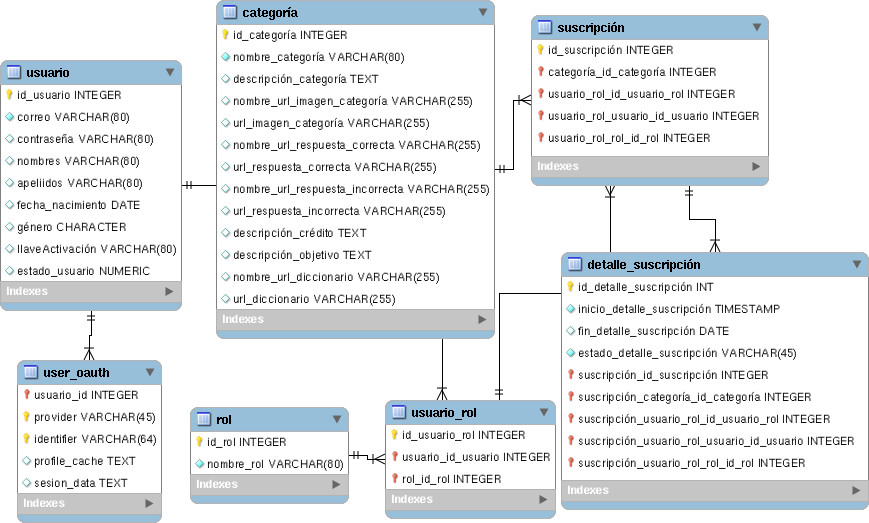
\includegraphics[scale=0.4]{modelSubscription}
	}
	\captionof{figure}{Modelo Subscripci\'{o}n Modelo de Datos}
	\source{fuente: (Elaboraci\'{o}n Propia)}
	\label{fig:Modelo Subscripci\'{o}n Modelo de Datos}
\end{minipage}

\subsection{M\'{o}dulo o componente}

En la Figura \ref{fig:Ventana emergente subscripci\'{o}n} se opta por 
subscripci\'{o}n por programa de aprendizaje (sub-categor\'{i}a), el
usuario debe autentificarse para poder subscribirse.

Se brinda dos opciones para la subscripci\'{o}n como ser: Primera Opci\'{o}n
Manual, la misma permite ingresar solo una direcci\'{o}n de correo sujeto a verificaci\'{o}n
Segunda Opci\'{o}n Red Social, Google, Facebook, Twitter. 

\begin{minipage}{1.0\textwidth}
	\centering
	\fbox{
		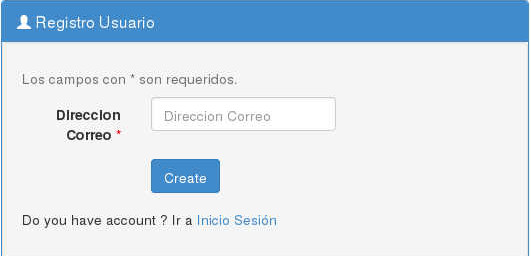
\includegraphics[scale=0.4]{modalSubscribe}
	}
	\captionof{figure}{Ventana emergente subscripci\'{o}n}
	\source{fuente: (Elaboraci\'{o}n Propia)}
	\label{fig:Ventana emergente subscripci\'{o}n}
\end{minipage}

En la Figura \ref{fig:Formulario de Autentificaci\'{o}n} una opci\'{o}n emergente
luego de pinchar sobre opci\'{o}n Inicio Sesi\'{o}n. Se Ingresa a Sistema con
los siguientes campos: Nombre Usuario, Contrase\~{n}a.

\begin{minipage}{1.0\textwidth}
	\centering
	\fbox{
		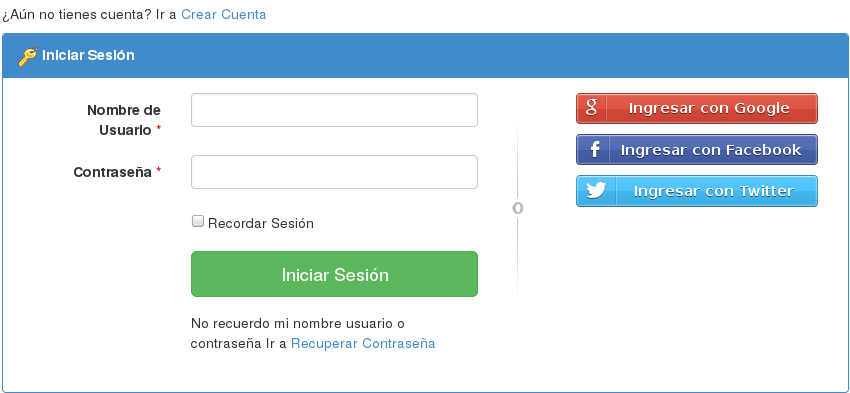
\includegraphics[scale=0.4]{login}
	}
	\captionof{figure}{Formulario de Autentificaci\'{o}n}
	\source{fuente: (Elaboraci\'{o}n Propia)}
	\label{fig:Formulario de Autentificaci\'{o}n}
\end{minipage}

En la Figura \ref{fig:Facebook OAuth Autenticatition} se facilita el Diagrama 
Secuencia en uso de un servicio externo, para facilitar un acceso, partiendo
de una cuenta v\'{a}lida dentro los usuarios en Facebook.

\begin{minipage}{1.0\textwidth}
	\centering
	\fbox{
		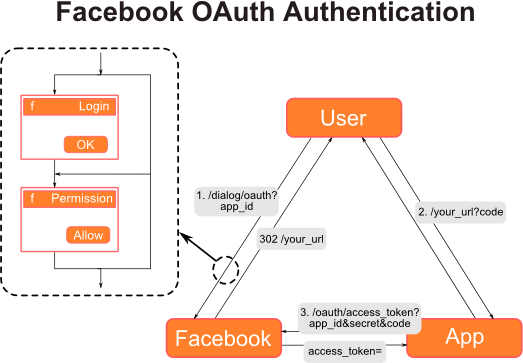
\includegraphics[scale=0.4]{oauthFacebook}
	}
	\captionof{figure}{Facebook OAuth Autenticatition}
	\source{fuente: facebookOAuth}
	\label{fig:Facebook OAuth Autenticatition}
\end{minipage}

En la Figura \ref{Aplicaciones de servidor web} se facilita el Diagrama Secuencia
en uso de un servicio externo, para facilitar un acceso, partiendo de una cuenta
v\'{a}lida dentro los usuarios en Google.

\begin{minipage}{1.0\textwidth}
	\centering
	\fbox{
		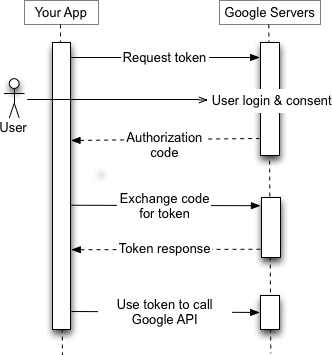
\includegraphics[scale=0.5]{oauth20Google}
	}
	\captionof{figure}{Aplicaciones de servidor web}
	\source{fuente: OAuth 2.0 Authorization Document}
	\label{Aplicaciones de servidor web}
\end{minipage}

En la Figura \ref{Aplicaci\'{o}n de solo autentificaci\'{o}n} se facilita el 
Diagrama Secuencia en uso de un servicio externo, para facilitar un acceso,
partiendo de una cuenta v\'{a}lida dentro los usuarios en Twitter.

\begin{minipage}{1.0\textwidth}
	\centering
	\fbox{
		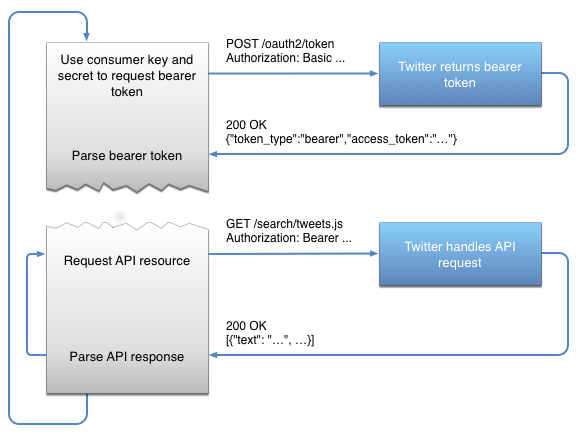
\includegraphics[scale=0.3]{oauth10Twitter}
	}
	\captionof{figure}{Aplicaci\'{o}n de solo autentificaci\'{o}n}
	\source{fuente: Auth Flow 1.0 model Document}
	\label{Aplicaci\'{o}n de solo autentificaci\'{o}n}
\end{minipage}

En la Figura \ref{Job Queue Architecture} se muestra la comunicaci\'{o}n de
componentes que interactuan para ejecutar un proceso en segundo plano, el mismo
debe ejecutarse en base fecha liberaci\'{o}n definida en un podcast al 
momento de el registro.   

\begin{minipage}{1.0\textwidth}
	\centering
	\fbox{
	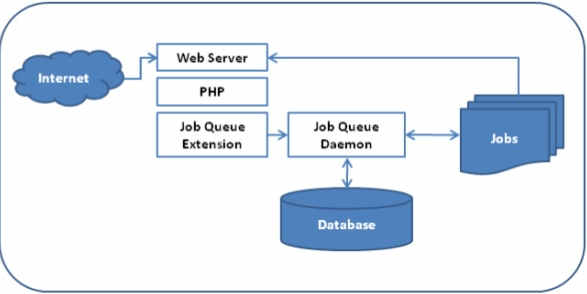
\includegraphics[scale=0.5]{jobQueue}
	}
	\captionof{figure}{Job Queue Architecture}
	\source{fuente:\cite{ossCamp2014}}
	\label{Job Queue Architecture}
\end{minipage}
	
\subsection{Implementaci\'{o}n}

Se define el siguiente Segmento C\'{o}digo donde se personaliza la subscripci\'{o}n
por programa de aprendizaje. El cual permite poder visualizar programas de 
aprendizaje habilitados sujetos a subscripci\'{o}n.

\begin{lstlisting}[language = PHP]
public function actionCustomRss($idCategory) {
ob_end_clean();
// turn off layout
$this->layout = false;
// add custom criteria
$criteria = new CDbCriteria;
$criteria->addCondition('t.category_id_category=:Column1');
$criteria->addCondition('t.category_id_category in (select 
i.category_id_category from interest as i) and t.content_status=
'.Yii::app()->params['stateContentAvailable']);
$criteria->select = 't.title,t.summary,t.date_leave';
$criteria->params = array(':Column1' => $idCategory);
$data = Content::model()->findAll($criteria);
// redirect view
$this->renderPartial('_viewItemChannel', array('data' => $data));
}
\end{lstlisting}

Se define por medio de contrab un shell sobre una distribuci\'{o}n linux 
especificar la funci\'{o}n asincrona permite ejecutar script ejecuci\'{o}n
de liberaci\'{o}n de podcast el cual realiza la comparaci\'{o}n de la fecha
actual con la fecha de liberaci\'{o}n.

\begin{lstlisting}[language = PHP]
public function run($args) {	
$jobs = $this->getJobs();
foreach ($jobs as $job) {
	Yii::log("Running - Job [".$job->title."] scheduled for "
	.$job->date_create,'info', 'jobprocessor');
    // set field available
    $job->content_status = Yii::app()->params['stateContentAvailable'];
    // save data
    $job->save();
    $this->sendMailSubscribed($job->category_id_category, 
    $job->user_id_user, $job->title, $job->summary);
}

}
\end{lstlisting}

\subsection{Problema/Soluci\'{o}n}

Se consideran las siguientes dificultades que surgieron para la implementaci\'{o}n
para el Servicio Agregador de Noticias.

\begin{itemize}

\item Generaci\'{o}n \'{u}nica de Modal respecto a Programa Aprendizaje 
(sub-categor\'{i}a)
\item Env\'{i}o de mensaje de notificaci\'{o}n de liberaci\'{o}n contenido tarea
en segundo plano. 

\end{itemize}

En la generaci\'{o}n de varias programas de aprendizaje sobre una lista con acceso a
una ventana modal sujeto subscripci\'{o}n, este identificador anteriormente
ten\'{i}a asignado siempre el mismo identificador del \'{u}ltimo programa.

\begin{enumerate}

\item \textbf{Generar \'{U}nico identificador por Modal}

Se define como mecanismo de soluci\'{o}n para generar un identidicador como ser:
Categor\'{i}a: Frances, Programa Aprendizaje: Frances B\'{a}sico. Categor\'{i}a:
Ingl\'{e}s, Programa Aprendizaje: Ingl\'{e}s B\'{a}sico. Categor\'{i}a: Quechua,
Programa Aprendizaje: Quechua B\'{a}sico, Quechua Psicosocial. Categor\'{i}a: Quechua,
Programa Aprendizaje: Fon\'{e}tica Quechua

\begin{lstlisting}[language = PHP]
<?php $this->beginWidget(
        'booster.widgets.TbModal', array(
    'id' => 'myModal' . $category_id,
));?>

<div class="modal-body">
    <div class="panel-body">
        <?php $this->renderPartial('//site/createRegisterSuscribe', 
        array('model_user' => $model_user)); ?>
    </div>
</div>

<?php $this->endWidget(); ?>
\end{lstlisting}

Se tubo problemas al momento de enviar la notificaci\'{o}n a las cuentas de correo
que se encuentran subscritos a un programa de aprendizaje, debido que el mensaje de 
correo contiene etiquetas propias de HTML \footnote{HTML: Es el lenguaje de marcado
est\'{a}ndar utilizado para crear p\'{a}ginas web y sus elementos forman los bloques
de construcci\'{o}n de todos los sitios web}

\item \textbf{Envio Mensajes}

Se define Segmento C\'{o}digo como la implementaci\'{o}n de envio de mail con la 
caracter\'{i}stica de que muestra el mensaje de correo sin p\'{a}gina maestra.

\begin{lstlisting}[language = PHP]
private function sendMailSubscribed($idCategory, $idUser,
 $title, $summary) {
$userRols = Category::model()->getRecentUserSubscribe($idCategory);
foreach ($userRols->categoryUserRol as $userRol) {
if ($idUser != $userRol->user_id_user) {
// set properties
$subject = Yii::app()->params['setSubjectContentRelease'];
$body = Yii::app()->params['setBodyContentRelease'] . $title . $summary
. Yii::app()->params['setBodyBelowContentRelease'] . 
Yii::app()->params['adminEmail'] . 
Yii::app()->params['setBodyBottomContentRelease'];
$to = $userRol->userIdUser->email;
// send mail
$mail = new YiiMailer();
//use "cron" view from views/mail
$mail->setBody($body);
$mail->setData(array('message' => $subject, 'name' => get_class($this),
'description' => 'Cron job', 'mailer' => $mail));
//render HTML mail, layout is set from config file or with 
//$mail->setLayout('layoutName')
$mail->render();
//set properties as usually with PHPMailer
$mail->From = Yii::app()->params['adminEmail'];
$mail->FromName = Yii::app()->params['fromNameConsole'];
$mail->Subject = $subject;
$mail->AddAddress($to);
// send
if ($mail->Send()) {
	// load the message succeed
    Yii::log(Yii::app()->params['succeedSendContentRelease']);
} else {
	// load the message wrong
    Yii::log(Yii::app()->params['wrongSendContenRelease']);
}
}
}
}    
\end{lstlisting}

\end{enumerate}

\section{Mecanismos de Transcripci\'{o}n}

Se desea poder integrar el reproductor de un Podcast con su propia conversaci\'{o}n
de tal forma se tenga un efecto de mayor compensi\'{o}n auditiva y visual.

Tambi\'{e}n se desea poder generar definici\'{o}n de palabras referentes a contenido
Podcast de forma textual.
 
\subsection{Tarjetas de Historias de Usuario}

% add user history card 59
\begin{minipage}[b]{\hsize}\centering
\begin{tabular}{|l|l|l|}
\hline
 & \textbf{Tarjeta Historia de Usuario} &  \\ \hline
ID Historia: 59 & \begin{tabular}[c]{@{}l@{}}Nombre: Gestionar\\ Karaoke transcripción \\ podcast\end{tabular} & Fecha: 09/05/2015 \\ \hline
\multicolumn{3}{|l|}{Rol: Tutor} \\ \hline
\begin{tabular}[c]{@{}l@{}}Modificación de Historia\\ Numero:\end{tabular} & Iteración Asignada: 14 & Prioridad en Negocio: Medio \\ \hline
Tiempo Estimado Inicial: 35 & Riesgo en Desarrollo: & Tipo de Historia: Funcional \\ \hline
\multicolumn{3}{|l|}{\begin{tabular}[c]{@{}l@{}}Descripción:\\ \\ Yo como usuario Tutor deseo tener un karaoke tal que me beneficie poder relacionar el reproductor\\ con la conversación del podcast.\\ \\ Para esto necesito: Tipo Traducción, Frase, Lenguage (Destino), Significado, Tiempo Inicio,\\ Tiempo Fin.\end{tabular}} \\ \hline
\multicolumn{3}{|l|}{\begin{tabular}[c]{@{}l@{}}Pre Condición:	\\ \\ Usuario Autentificado.\end{tabular}} \\ \hline
\multicolumn{3}{|l|}{Post Condición:} \\ \hline
\multicolumn{3}{|l|}{\begin{tabular}[c]{@{}l@{}}Como Probarlo:\\ \\ Se tiene que pinchar sobre botón play reproductor\\
pinchar dos veces sobre el boton Mostrar/Ocultar\\ Transcripción, para poder apreciar la transcripción además de una \\
 traducción a un lenguaje destino.\end{tabular}} \\ \hline
\begin{tabular}[c]{@{}l@{}}.....................................................\\ Msc. Lic. Vladimir Costas Juaregui\\ PROJECT MANAGER\end{tabular} & \begin{tabular}[c]{@{}l@{}}..........................................\\ Lic. Manuel Camacho Arce\\ PRODUCT OWNER\end{tabular} & \begin{tabular}[c]{@{}l@{}}.........................................\\ Juan Omar Huanca Balboa\\ SCRUMMASTER\end{tabular} \\ \hline
\end{tabular}
\captionof{table}{Tarjeta Historia de Usuario 60}
\source{fuente: (Elaboraci\'{o}n Propia)}
\end{minipage}

% add user history card 60
\begin{minipage}[b]{\hsize}\centering
\begin{tabular}{|l|l|l|}
\hline
 & \textbf{Tarjeta Historia de Usuario} &  \\ \hline
ID Historia: 60 & \begin{tabular}[c]{@{}l@{}}Nombre: Gestionar \\ Diccionario podcast\end{tabular} & Fecha: 09/05/2015 \\ \hline
\multicolumn{3}{|l|}{Rol: Tutor} \\ \hline
\begin{tabular}[c]{@{}l@{}}Modificación de Historia\\ Numero:\end{tabular} & Iteración Asignada: 14 & Prioridad en Negocio: Medio \\ \hline
Tiempo Estimado Inicial: 30 & Riesgo en Desarrollo: & Tipo de Historia: Funcional \\ \hline
\multicolumn{3}{|l|}{\begin{tabular}[c]{@{}l@{}}Descripción:\\ \\ Yo como usuario Tutor deseo gestionar un diccionario tal que me beneficie poder \\ definir términos por cada Episodio.\\ \\ Para esto necesito: Tipo Traducción, Frase, Lenguage (Destino), Significado.\end{tabular}} \\ \hline
\multicolumn{3}{|l|}{\begin{tabular}[c]{@{}l@{}}Pre Condición:	\\ \\ Usuario Autentificado.\end{tabular}} \\ \hline
\multicolumn{3}{|l|}{Post Condición:} \\ \hline
\multicolumn{3}{|l|}{\begin{tabular}[c]{@{}l@{}}Como Probarlo:\\ \\ Se tiene que situar sobre detalle Podcast, para luego pinchar sobre la\\ segunda opción Definición Diccionario dentro del Tab de opciones.\end{tabular}} \\ \hline
\begin{tabular}[c]{@{}l@{}}.....................................................\\ Msc. Lic. Vladimir Costas Juaregui\\ PROJECT MANAGER\end{tabular} & \begin{tabular}[c]{@{}l@{}}..........................................\\ Lic. Manuel Camacho Arce\\ PRODUCT OWNER\end{tabular} & \begin{tabular}[c]{@{}l@{}}.........................................\\ Juan Omar Huanca Balboa\\ SCRUMMASTER\end{tabular} \\ \hline
\end{tabular}
\captionof{table}{Tarjeta Historia de Usuario 60}
\source{fuente: (Elaboraci\'{o}n Propia)}
\end{minipage}

\subsection{Modelo de Datos}

En la Figura \ref{fig:Modelo Transcripci\'{o}n}	se define el modelo parcial de 
Base de Datos de un mecanismo de transcripci\'{o}n.

\begin{minipage}{1.0\textwidth}
	\centering
	\fbox{
		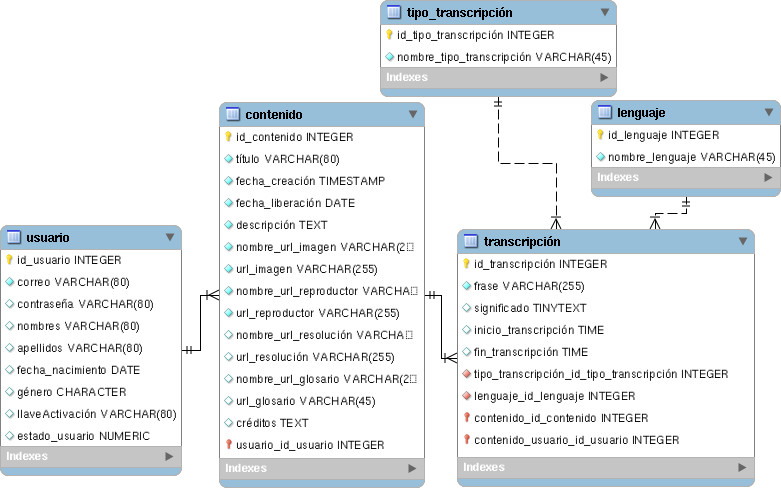
\includegraphics[scale=0.35]{modelTranslation}
	}
	\captionof{figure}{Modelo Transcripci\'{o}n}
	\source{fuente: (Elaboraci\'{o}n Propia)}
	\label{fig:Modelo Transcripci\'{o}n}
\end{minipage}

\subsection{M\'{o}dulo o componente}

En la Figura \ref{fig:Diagrama Estados Karaoke} se define la estructura la
que se tom\'{o} en cuenta para la elaboraci\'{o}n del subtitulado de una frase
para definir tanto para el subtitulado origen, subtitulado destino, tiempos 
inicio, tiempo fin de una frase.

\begin{minipage}{1.0\textwidth}
	\centering
	\fbox{
		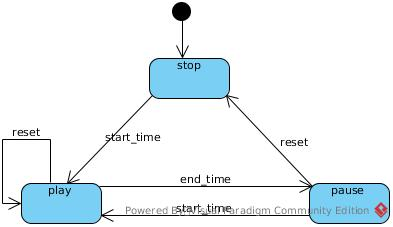
\includegraphics[scale=0.6]{stateLyric}
	}
	\captionof{figure}{Diagrama Estados Karaoke}
	\source{fuente: (Elaboraci\'{o}n Propia)}
	\label{fig:Diagrama Estados Karaoke}
\end{minipage}

En la Figura \ref{fig:Formulario Registro Transcripci\'{o}n} se representa los 
distintos campos necesarios para realizar el subtitulado del lenguaje origen, 
lenguaje destino, tomando en cuenta el reproductor del podcast que es fundamental
para la asignaci\'{o}n.

\begin{minipage}{1.0\textwidth}
	\centering
	\fbox{
		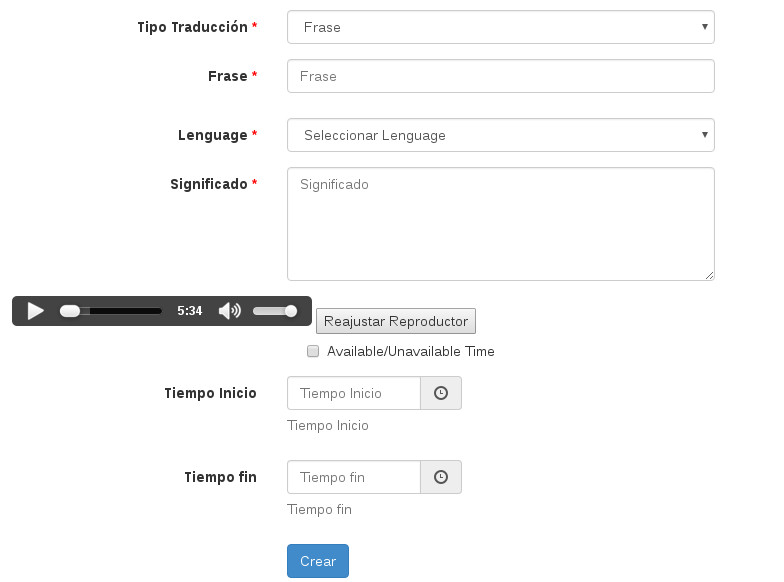
\includegraphics[scale=0.4]{formTranslation}
	}
	\captionof{figure}{Formulario Registro Transcripci\'{o}n}
	\source{fuente: (Elaboraci\'{o}n Propia)}
	\label{fig:Formulario Registro Transcripci\'{o}n}
\end{minipage}


\subsection{Implementaci\'{o}n}

Se define la funcionalidad para obtener dos listas en los siguiente: 
Transcripci\'{o}n lenguaje origen propio podcast, Transcripci\'{o}n
a un lenguaje destino para mayor comprension sobre los rol Autorregulado.

\begin{lstlisting}[]
$(document).ready(function () {
try {
// get object audio player
var myPlayer = document.getElementById("audio-player");
// flag for run one time
var flag = false;
<?php if (isset($model_translation)): ?>
// add event play listener
myPlayer.addEventListener("play", function () {
// verify no change flag
if (!flag) {
// get property through ajax
$.ajax({
type: "POST",
url: "<?php echo CController::createUrl('Translation/getItemSentences');
 ?>",
data: {
idTypeTranslation: "<?php echo 
Yii::app()->params['idTypeTranslationSentence']; ?>",
idContent: "<?php echo 
Yii::app()->getRequest()->getParam('id_content'); ?>",
idUser: "<?php echo 
Yii::app()->getRequest()->getParam('user_id_user'); ?>",
idLanguage: "<?php echo 
$model_translation->language_id_language; ?>"
},
dataType: "html",
success: function (data) {
var div = document.getElementById("idSentence");
div.innerHTML = data;
}
});
// get property through ajax
$.ajax({
type: "POST",
url: "<?php echo CController::createUrl(
'Translation/getItemMeanings'); ?>",
data: {
idTypeTranslation: "<?php echo Yii::app()->params[
'idTypeTranslationSentence']; ?>",
idContent: "<?php echo 
Yii::app()->getRequest()->getParam('id_content'); ?>",
idUser: "<?php echo 
Yii::app()->getRequest()->getParam('user_id_user'); ?>",
idLanguage: "<?php echo 
$model_translation->language_id_language; ?>"
},
dataType: "html",
success: function (data) {
var div = document.getElementById("idMeaning");
div.innerHTML = data;
}
});
// change flag
flag = true;
// call function for show karaoke
play(myPlayer);
}
}, false);
<?php endif; ?>
} catch (err) {
    console.log(err);
}
});
\end{lstlisting}

Se define la siguiente funci\'{o}n, donde se realiza las acciones necesarias para
mostrar/ocultar el subtitulado del lenguage origen sujeto a la acci\'{o}n de un 
bot\'{o}n.  

\begin{lstlisting}[]
function play(myPlayer) {
var controlDuplicate = [];
myPlayer.ontimeupdate = function () {
// get currentTime player
var currentTimePhrase = myPlayer.currentTime;
// identifier for start_translation, end_translation
var currentIDStart = "";
var currentIDEnd = "";
// time converter min:seg
var timeConvert = "";
//convert from seg:miliseg to min:seg
var hr = Math.floor(currentTimePhrase / 3600);
var min = Math.floor((currentTimePhrase - (hr * 3600)) / 60);
var sec = Math.floor(currentTimePhrase - (hr * 3600) - (min * 60));
// if min is less 10 add 0
if (min < 10) {
    min = "0" + min;
}
// if sec is less 10 add 0
if (sec < 10) {
    sec = "0" + sec;
}
timeConvert = min + ':' + sec + ':00';
if (controlDuplicate.length == 0) {
    controlDuplicate.push(timeConvert);
$('#idSentence li').filter(':not([start_time_translation]), \n\
    [start_time_translation="' + timeConvert + '"]').addClass(
    'sentence_show');
$('#idMeaning li').filter(':not([start_time_translation]), \n\
    [start_time_translation="' + timeConvert + '"]').addClass(
    'sentence_show');
} else if (controlDuplicate[controlDuplicate.length - 1] != timeConvert) {
    controlDuplicate.push(timeConvert);
$('#idSentence li').filter(':not([start_time_translation]), \n\
    [start_time_translation="'+ timeConvert + '"]').addClass(
    'sentence_show');
$('#idSentence li').filter(':not([start_time_translation]), \n\
    [end_time_translation="' + timeConvert + '"]').removeClass(
    'sentence_show');
$('#idMeaning li').filter(':not([start_time_translation]), \n\
    [start_time_translation="' + timeConvert + '"]').addClass(
    'sentence_show');
$('#idMeaning li').filter(':not([start_time_translation]), \n\
    [end_time_translation="' + timeConvert + '"]').removeClass(
    'sentence_show');
}
};
}       
\end{lstlisting}

\subsection{Problema/Soluci\'{o}n}

Se considera las siguientes dificultades que surgieron para la implementaci\'{o}n
para Mecanismos de Transcripci\'{o}n.

\begin{itemize}

\item Definici\'{o}n de segundos, minutos para tiempo inicio, tiempo final frase inicial.
\item Definici\'{o}n de campos: tiempo inicio, tiempo final para la frases.

\end{itemize}

\begin{enumerate}

\item \textbf{Definici\'{o}n }

La siguiente funcionalidad se debe para realizar el control de la definici\'{o}n
de campos tiempo inicio, tiempo fin en base al reproductor definido para el podcast,
tomando en cuenta restricciones de opciones.

\begin{lstlisting}[]
$(document).ready(function () {
try {
var myPlayer = document.getElementById("playerMyTranslation");
myPlayer.addEventListener("play", function () {
var status_start_translation = document.getElementById(
    'start_translation').disabled;
if (!status_start_translation) {
    var second_start_translation = Math.floor(myPlayer.
    currentTime % 60);
if (second_start_translation < 10) {
    second_start_translation = "0" + 
    second_start_translation;
}
var minute_start_translation = Math.floor((myPlayer.
        currentTime / 60) % 60);
if (minute_start_translation < 10) {
    minute_start_translation = "0" + 
    minute_start_translation;
}
document.getElementById('start_translation').value = 
    minute_start_translation +':' + second_start_translation;
}
}, false);

myPlayer.addEventListener("pause", function () {
var status_end_translation = document.getElementById(
        'end_translation').disabled;
if (!status_end_translation) {
var second_end_translation = Math.floor(myPlayer.currentTime 
    % 60);
if (second_end_translation < 10) {
    second_end_translation = "0" + second_end_translation;
}
var minute_end_translation = Math.floor((myPlayer.currentTime 
    / 60) % 60);
if (minute_end_translation < 10) {
    minute_end_translation = "0" + minute_end_translation;
}
document.getElementById('end_translation').value = 
    minute_end_translation + ':' + second_end_translation;
}
}, false);
} catch (err) {
    console.log(err);
}
});
\end{lstlisting}

\item \textbf{Frase }

La siguiente funcionalidad se debe para realizar el reset de los campos tiempo
inicio, tiempo fin, como del reproductor a un estado inicial.

\begin{lstlisting}[]
function resetPlayer() {
var status_start_translation = document.getElementById(
    'start_translation').disabled;
var status_end_translation = document.getElementById(
    'end_translation').disabled;
var myPlayer = document.getElementById("playerMyTranslation");
if (!status_start_translation && !status_end_translation) {
    if (myPlayer.play) {
    myPlayer.currentTime = 0;
    // set start translation
    document.getElementById('start_translation').value = 0;
    // set end translalation
    document.getElementById('end_translation').value = 0;
    }
}
}
\end{lstlisting}

\end{enumerate}